\chapter{Mesurer l'impact de Charcot \textit{via} l'extraction des termes médicaux : quelle approche adopter ?}
\minitoc
\label{chap:resultats}

Ce chapitre présente les expérimentations réalisées dans le cadre des évaluations quantitatives et qualitatives de l'extraction des termes médicaux, considérés comme des vecteurs potentiels de l'influence des pratiques de Charcot. Nous abordons dans un premier temps les modalités de fouille avancée appliquée à nos deux corpus à travers des outils \textsc{OBVIE} et \textsc{TextPair} (section \ref{sect:obvie_textpair}), développés par l'équipe-projet \textsc{ObTIC}, en exposant à la fois leurs limites, ainsi que les stratégies mobilisées pour améliorer la qualité des extractions. Dans cette perspective, trois types de méthodes d'extraction terminologique ont été testés pour l'identification de phrases-clés :
\begin{enumerate}
	\item des approches basées sur des règles linguistique : outil \texttt{TermSuite} (section \ref{sect:termsuite})
	\item des approches statistiques, incluant les métriques \textsc{TF-IDF} et \textsc{BM25} (section \ref{sect:methodo_stat})
	\item des techniques d'apprentissage profond, à l'aide des librairies \texttt{keybert} et \texttt{keyphrase\allowbreak-vectorizers} (section \ref{sect:deep_learning})
\end{enumerate}


Lors de l'évaluation des performances de ces techniques, nous avons tenté, autant que faire se peut, de prendre en compte les synonymes de ces termes présentés dans le tableau \ref{tab:contributions_charcot}, afin d'introduire une plus grande souplesse dans l'interprétation des résultats. À titre d'exemple, les scores attribués aux termes synonymes tels que \textit{paralysie agitante} et \textit{maladie de Parkinson} sont examinés, et le score le plus élevé est retenu pour représenter la pathologie concernée. La comparaison des résultats obtenus par ces différentes approches permet d'évaluer les performances, depuis les méthodes classiques jusqu'aux techniques les plus avancées de l'état de l'art. À ces expérimentations s'ajoute une analyse de l'impact de l'entité \texttt{Jean-Martin Charcot}, calculé à l'aide de l'outil Rankingdom (section \ref{sect:rankingdom}).
Dans un second temps, les résultats obtenus feront l'objet d'une analyse qualitative (section \ref{sect:eval_quali}), afin d'apporter une lecture plus approfondie et nuancée de notre étude.
%+ visualisation des méthodes appliquées aux termes sous forme des diagrammes de barres
\section{Exploration du corpus Charcot : \textsc{OBVIE} et \textsc{TextPair}}
\label{sect:obvie_textpair}
Une première exploration de notre corpus d'étude, réalisée à l'aide de l'application \textsc{OBVIE}, a permis d'identifier plusieurs catégories de mots dits \og{}pleins\fg{} (sémantiquement chargés) : substantifs, noms propres, verbes, adjectifs et adverbes. Pour chacun de ces mots, l'application a calculé les statistiques globales sous forme des fréquences absolues et relatives, ainsi que des scores issus de méthodes d'analyse plus avancées telles que \textsc{TF-IDF}, \textsc{BM25} (détaillées dans la section \ref{sect:methodo_stat} ; les scores ne sont cependant pas normalisés dans \textsc{OBVIE}), le test du \textsc{$\chi$2} et le Test \textsc{G} (angl. \textit{G-test}). Pour chaque paramètre appliqué, \textsc{OBVIE} génère une liste de 499 mots. 

%quasi exclusivement constituée d'unigrammes. Nous retrouvons exceptionnellement les mots composés, tels que \textit{maladie mentale}, \textit{Société de biologie} ou \textit{rendre compte}, mais ce qui empêche l'extraction des termes plus pertinents pour l'analyse

exemples....
Bien que la typologie des mots 

Cependant, l'application ne permet pas de quantifier la pertinence des expressions polylexicales, soit les n-grammes de mots, très fréquentes dans les deux corpus et dont la décomposition entraînerait une perte d'information (p. ex. le terme polysémique \og{}bulbe\fg{} qui a une valeur spécifique dans l'expression figée \textit{bulbe rachidien}). En observant la figure \ref{fig:bulbe}, nous constatons que l'abscisse donne l'information sur les dates de publication des ouvrages compris dans les corpus, alors que l'ordonnée indique le nombre d'occurrences par million de mots, soit \textit{parties par million} (\textit{ppm})\footnote{\textit{Cf.} le guide d'utilisation d'\textsc{OBVIE} détaillé : \url{https://obtic.huma-num.fr/obvie//static/aide.html}.}. 
\begin{figure}[!ht]
    \centering
    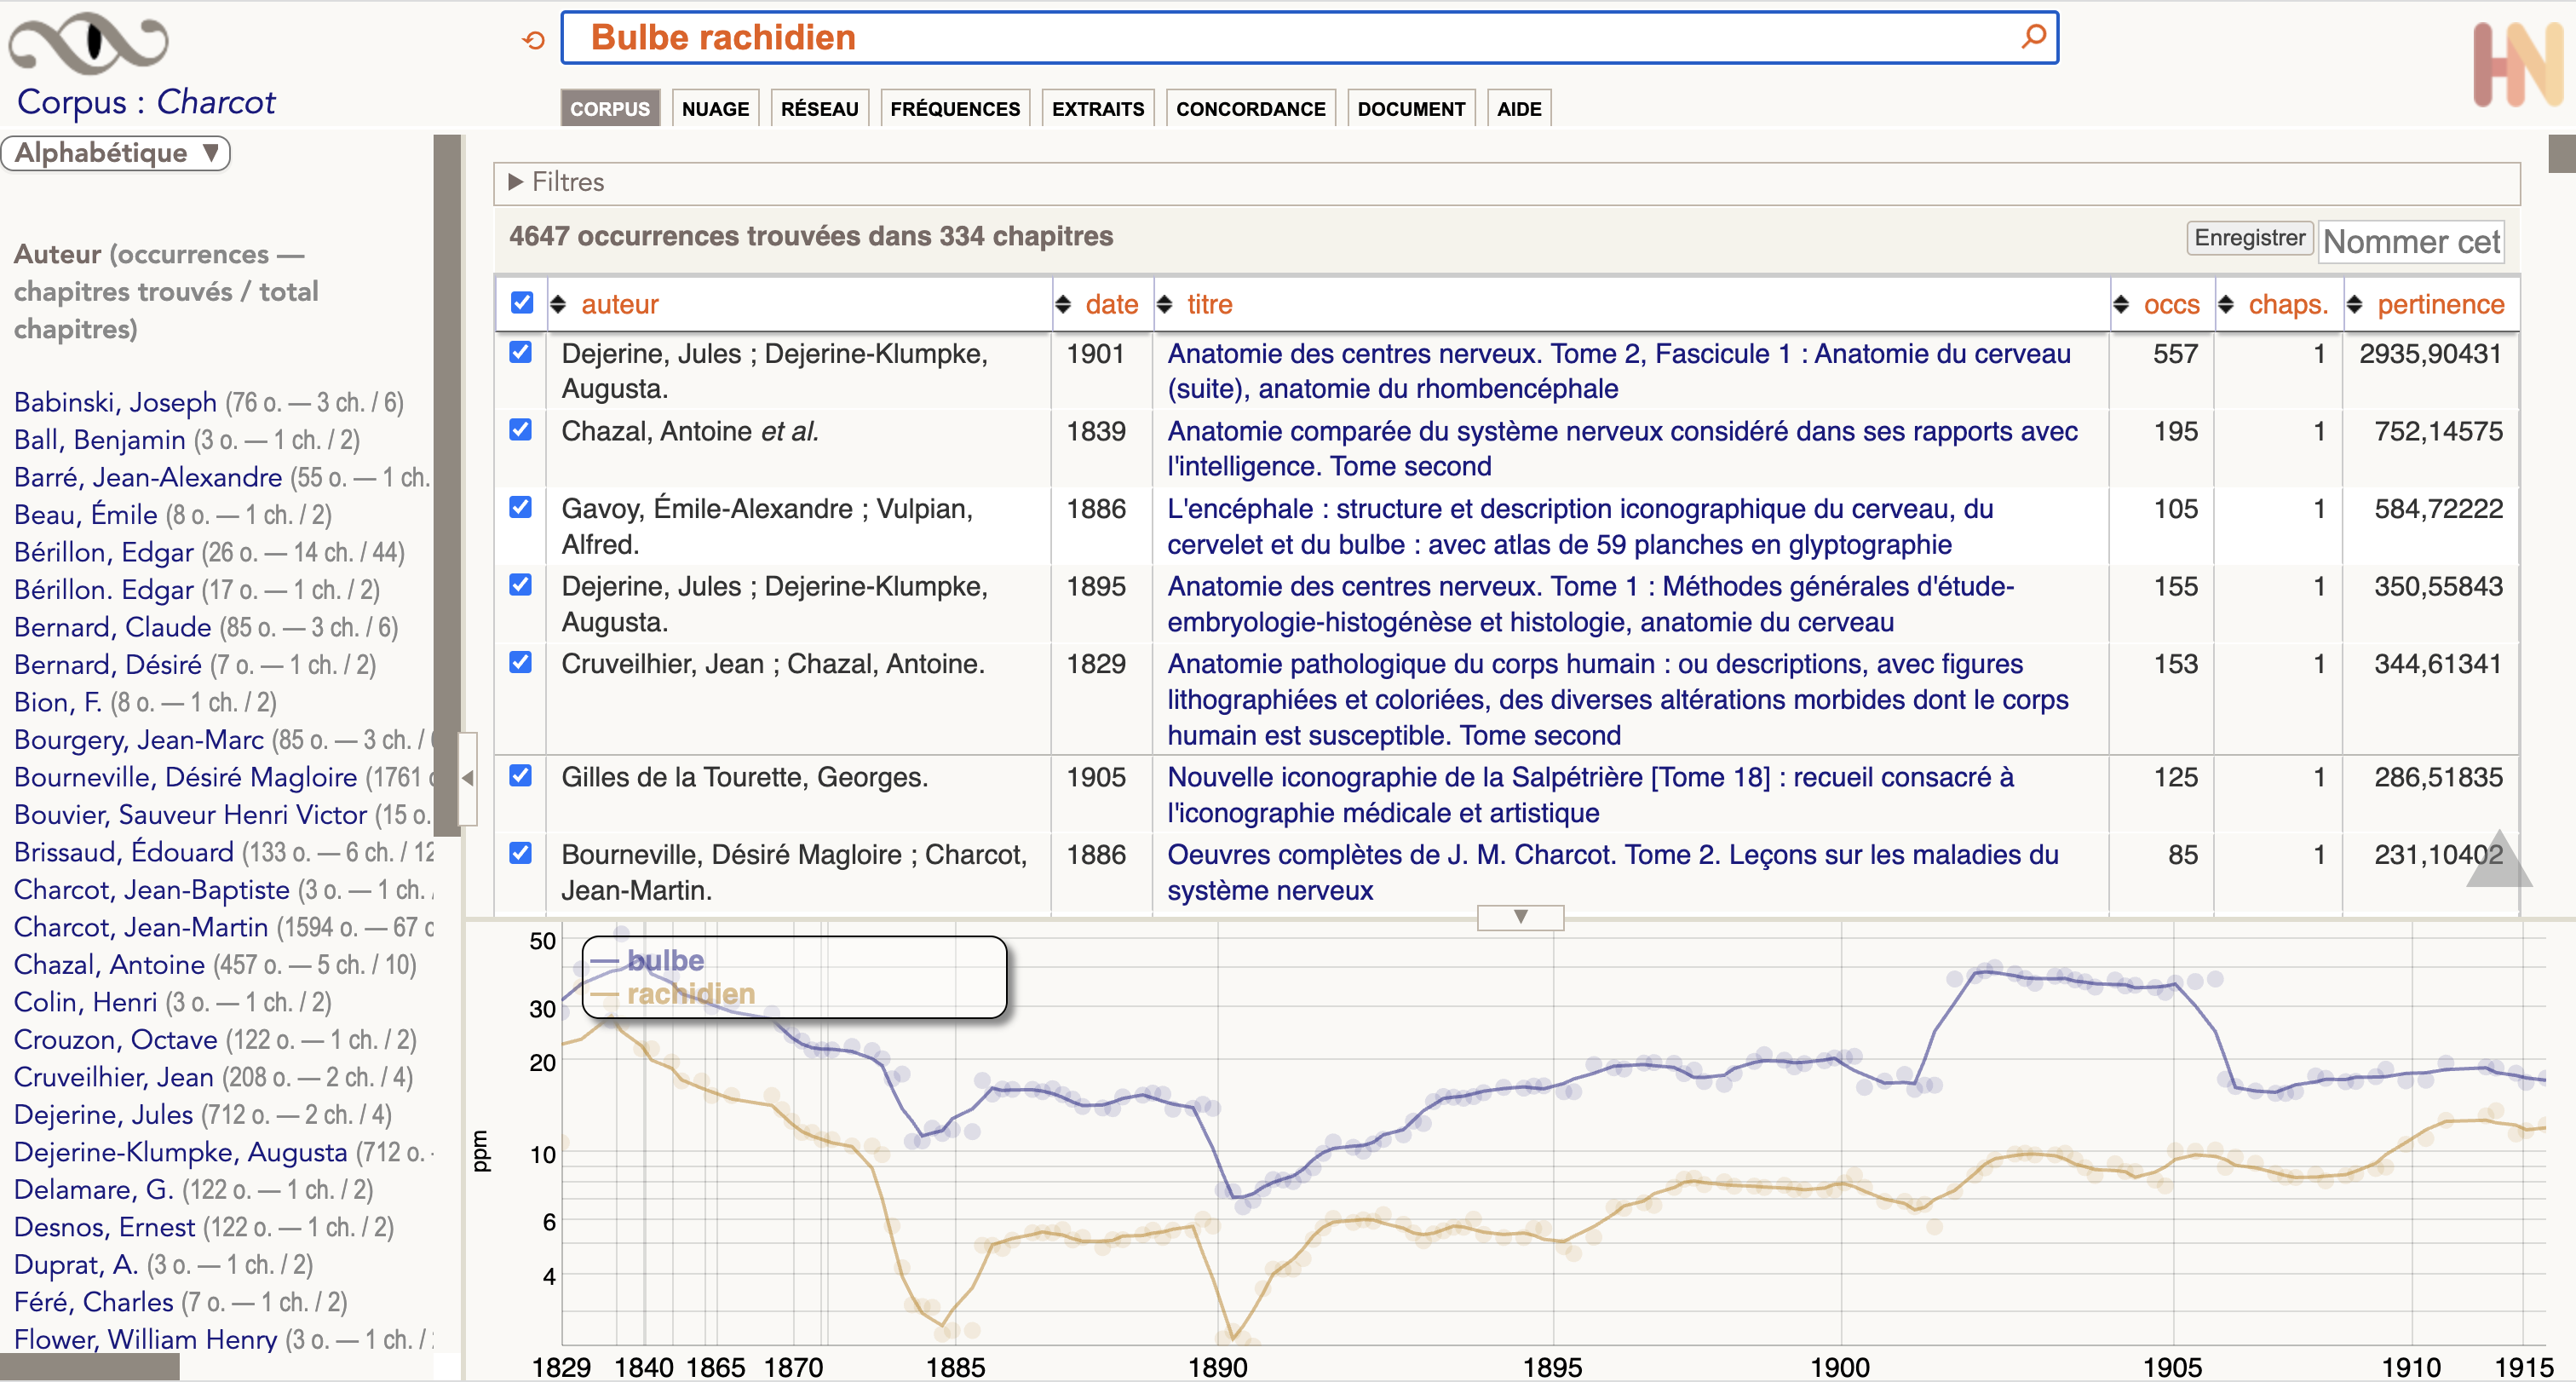
\includegraphics[width=1\textwidth]{img/bulbe_rachidien_mini.png}
    \caption{Distribution des fréquences des tokens avec la frise chronologique pour ceux constituant l'expression \og{}bulbe rachidien\fg{} (issus du corpus \og{}Charcot\fg{} et du corpus \og{}Autres\fg{}) dans le logiciel OBVIE.
    % Pour raison de visibilité, l'image originale a été agrandie, ce qui a entraîné le rapprochement des années sur l'axe de l'abscisse.
    }
    \label{fig:bulbe}
\end{figure}

Le moteur de recherche \textsc{OBVIE} permet également de repérer des textes similaires par ordre de pertinence à partir des termes en commun. 

D'autre part, l'algorithme \textsc{TextPair} génère une liste de passages similaires, c'est-à-dire les séquences de mots qui se chevauchent (n-grammes de mots) pour chaque texte, en comparant ensuite ces résultats avec ceux de séquences dans d'autres textes. Concernant l'alignement des séquences similaires aux deux corpus, \textsc{TextPair} nous a permis, par une lecture attentive, de faire des comparaisons entre les textes et de rechercher des termes au sein des passages similaires, malgré le nombre de résultats assez conséquent (\textit{cf}. la figure \ref{fig:textpair}). En raison de sa capacité de détecter les passages similaires, notamment les citations directes, les plagiats ou les réemplois, ce logiciel, ainsi qu'un autre logiciel de détection de plagiat, peuvent nous servir de \textit{baseline} pour comparer leurs résultats avec ceux proposés dans la partie \ref{methodo_stat}.

\begin{figure}[!ht]
    \centering
    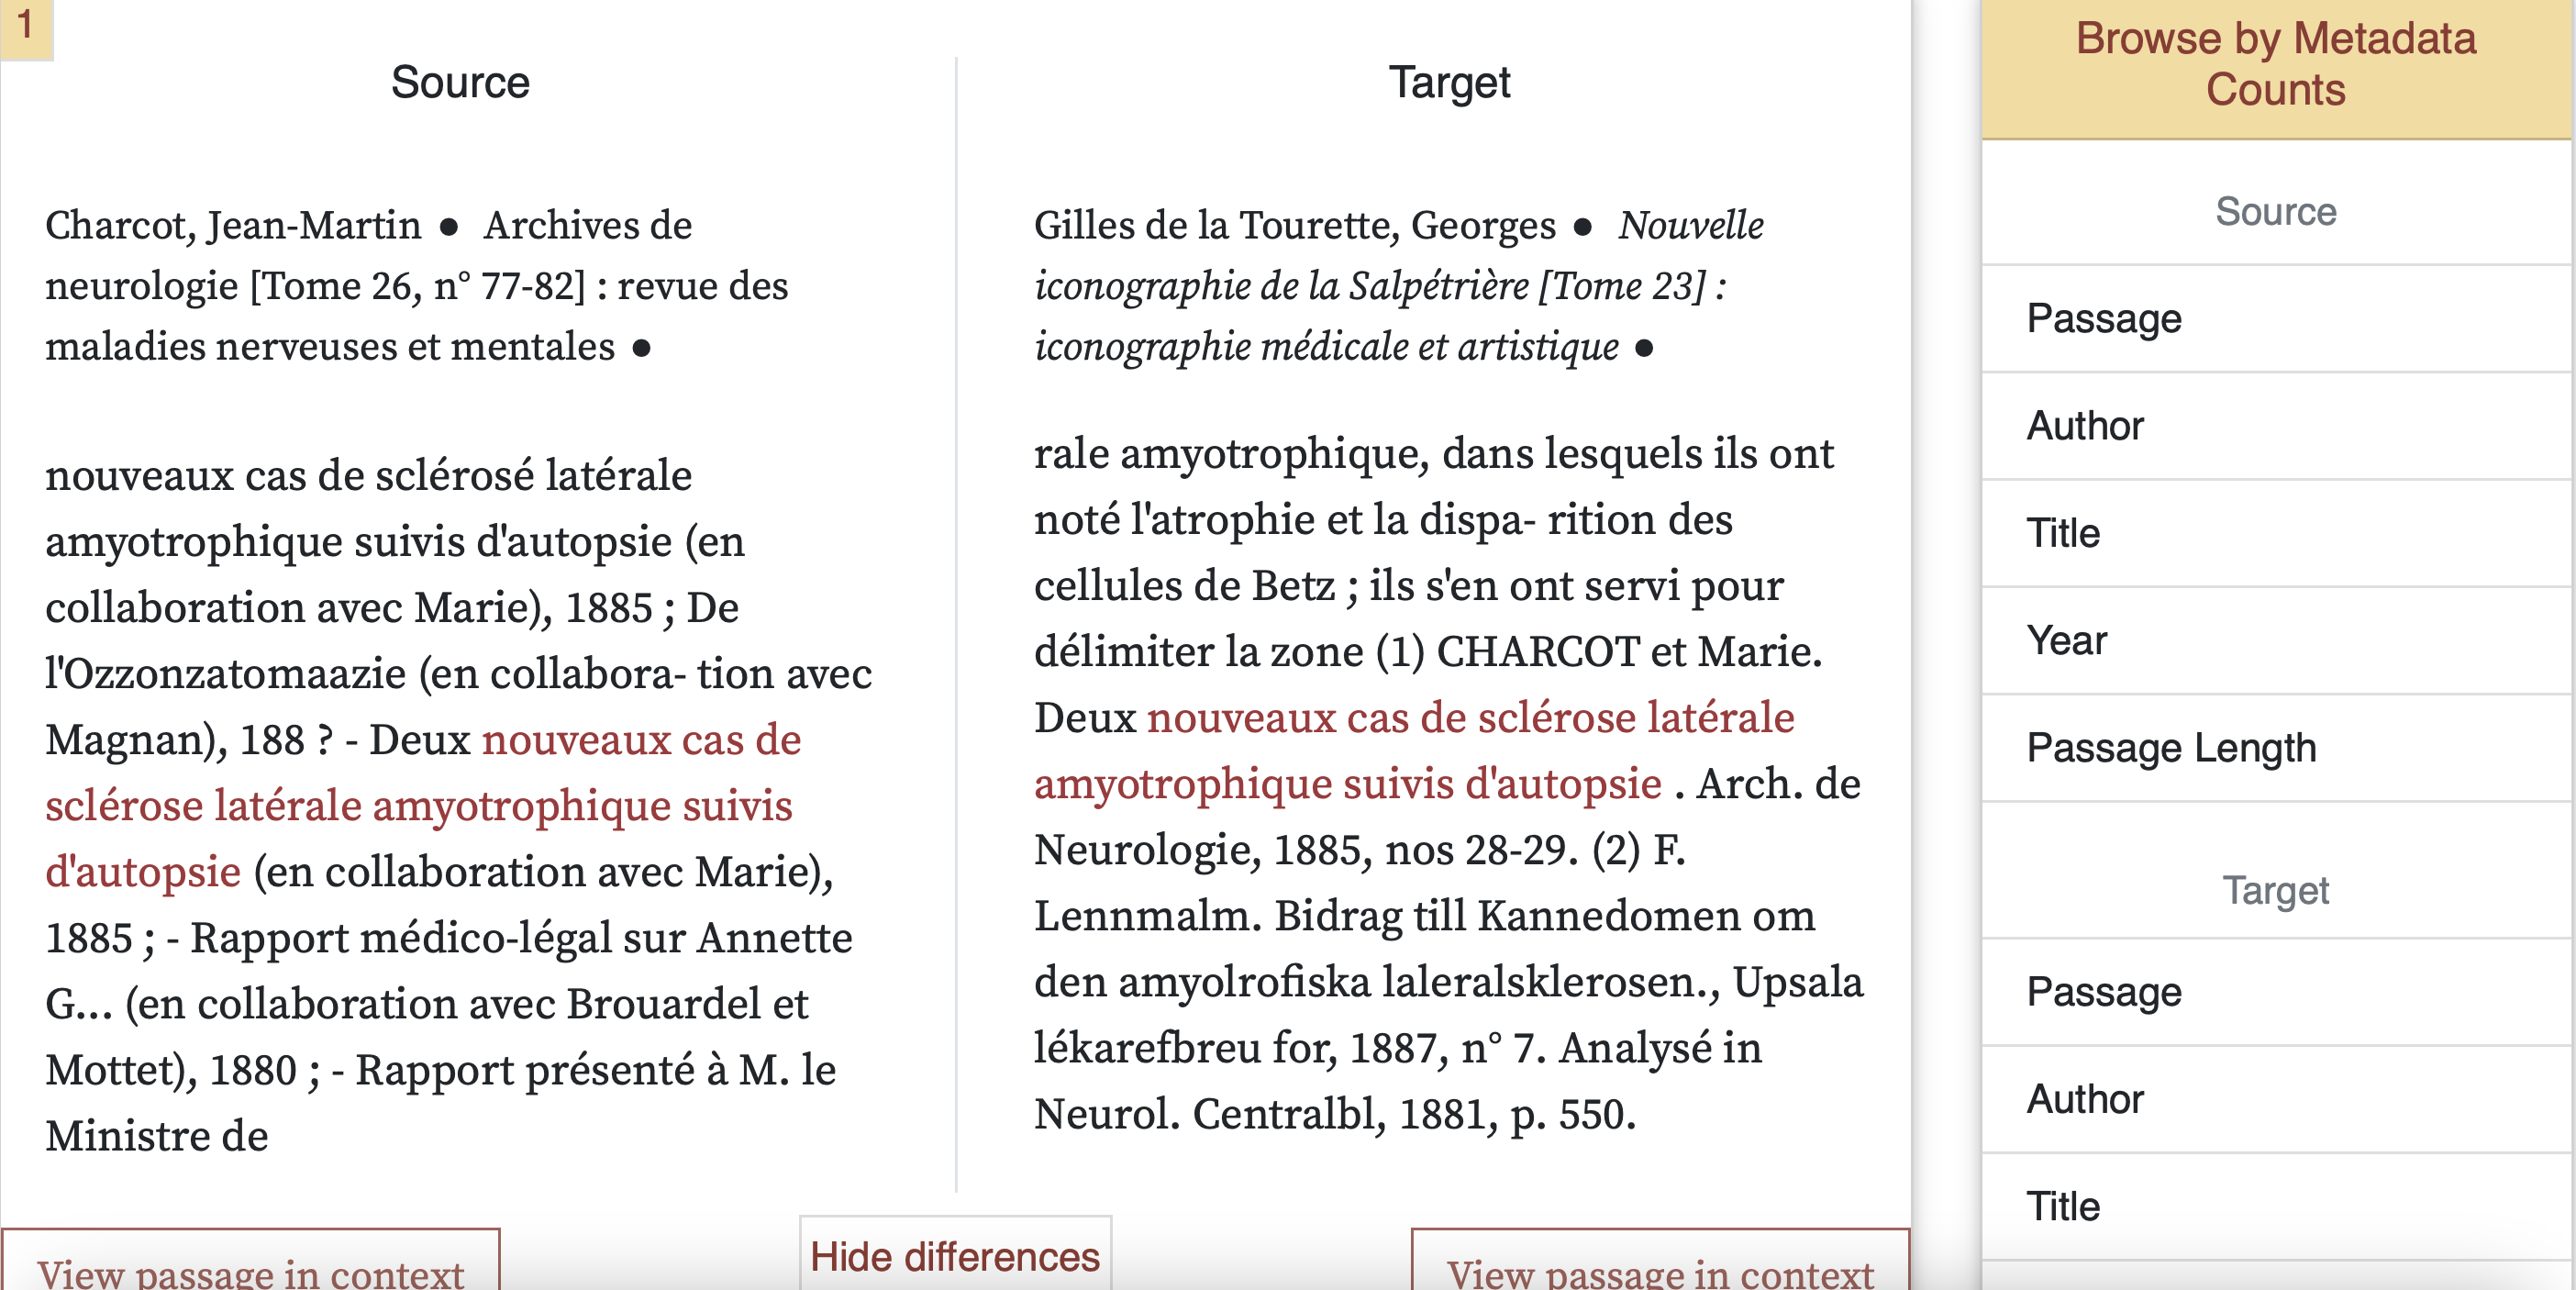
\includegraphics[width=1\textwidth]{img/textpair.png}
    \caption{Alignement et comparaison d'un texte de Charcot à celui de Georges Gilles de la Tourette (le seul résultat) en lançant la requête \textit{sclérose latérale amyotrophique}.}
    \label{fig:textpair}
\end{figure}

\section{Extraction de la terminologie : approche linguistique}
\label{sect:termsuite}
Dans le cadre de l'approche linguistique de l'extraction terminologique, nous avons tenté d'utiliser l'outil \texttt{TermoStat}. Bien que le traitement d'un échantillon minuscule des corpus (1-2 documents) ait pu se terminer avec succès, le passage à l'échelle de l'intégralité des corpus n'a pas été possible en raison des limitations citées dans la section \ref{termes}. Même en respectant la limite du corpus de 30 Mo, le traitement a été extrêmement chronophage, sans pour autant générer aucun résultat après plusieurs jours de calcul. En revanche, l'utilisation de l'outil \texttt{TermSuite} s'est avéré comme un moyen alternatif bien plus efficace pour générer les résultats souhaités, étant donné que le traitement de chaque corpus a duré environ une vingtaine de minutes\footnote{Les résultats sont disponibles dans le dépôt GitHub \url{https://github.com/ljpetkovic/Charcot\_TermSuite}}. Nous disposons de deux tableaux issus de l'extraction des termes uniques correspondant aux deux corpus, ainsi que de leurs diverses caractéristiques et mesures statistiques (motifs syntaxiques des parties du discours, fréquences brute et documentaire, \textsc{TF-IDF}, spécificité$\dots$). Concernant les motifs syntaxiques, nous en avons extrait 6 types, marqués par leurs étiquettes \texttt{TreeTagger} comme illustré dans le tableau \ref{tab:POS_tags}. 
\begin{table}[h]
	\centering
	\begin{tabular}{c|c}
		Étiquette & Signification \\\hline
		\textsc{A} & \texttt{adjectif}\\
		\textsc{N} & \texttt{nom}\\ 
		\textsc{N A} & \texttt{nom + adjectif}\\
		\textsc{N A A} & \texttt{nom + adjectif + adjectif}\\
		\textsc{N P N} & \texttt{nom + préposition + nom}\\
		\textsc{R} & \texttt{adverbe}
	\end{tabular}
	\caption{Étiquettes \texttt{TreeTagger} extraites avec \texttt{TermSuite}, accompagnées de leurs significations.}
	\label{tab:POS_tags}
\end{table} 

Le tableau \ref{tab:repartition_POS} montre les motifs syntaxiques extraits, avec leurs fréquences absolues (nombres d'occurrences extraites), leurs fréquences relatives (pourcentages de toutes les étiquettes extraites), avec des exemples des termes représentatifs correspondant à chaque motif.
\begin{table}[h]
	\centering
	\resizebox{\textwidth}{!}{
		\begin{tabular}{|lrrr|rrl|}
			\hline\hline
			\rowcolor{gray!10}\multicolumn{4}{|c|}{Corpus Charcot}                                                                    & \multicolumn{3}{|c|}{Corpus Autres}                               \\ \hline
			\multicolumn{1}{|c|}{Motif POS}      & \multicolumn{1}{c|}{Effectif} & \multicolumn{1}{c|}{Fréq. relat. (\%)} & \multicolumn{1}{c|}{Exemple} & \multicolumn{1}{c|}{Effectif} & \multicolumn{1}{c|}{Fréq. relat. (\%)} & \multicolumn{1}{c|}{Exemple}\\ \hline
			\rowcolor{yellow!30}\multicolumn{1}{|c|}{\textsc{N}}              & \multicolumn{1}{r|}{261}               & \multicolumn{1}{r|}{52,10}                   & \multicolumn{1}{c|}{\textit{hystérie}} & \multicolumn{1}{r|}{271}               & \multicolumn{1}{r|}{54,20} & \multicolumn{1}{c|}{\textit{somnambule}}                  \\ \hline
			\multicolumn{1}{|c|}{\textsc{A}}              & \multicolumn{1}{r|}{151}               &  \multicolumn{1}{r|}{30,14}                   & \multicolumn{1}{c|}{\textit{cérébral}} & \multicolumn{1}{r|}{149}               & \multicolumn{1}{r|}{29,80}      &   \multicolumn{1}{c|}{\textit{hypnotique}}          \\ \hline
			\multicolumn{1}{|c|}{\textsc{N A}}            & \multicolumn{1}{r|}{73}                & \multicolumn{1}{r|}{14,57}                   &
			\multicolumn{1}{c|}{\textit{système nerveux}} 	& \multicolumn{1}{r|}{73}                & \multicolumn{1}{r|}{14,60}       	&
			\multicolumn{1}{c|}{\textit{lame médullaire}}            \\ \hline
			\multicolumn{1}{|c|}{\textsc{N P N}}          & \multicolumn{1}{r|}{12}                & \multicolumn{1}{r|}{2,40}                    &
			\multicolumn{1}{c|}{\textit{cas de folie}} &
			\multicolumn{1}{r|}{6}                 & \multicolumn{1}{r|}{1,20}   &
			\multicolumn{1}{c|}{\textit{scissure de sylvius}}                 \\ \hline
			\multicolumn{1}{|c|}{\textsc{N A A}}          & \multicolumn{1}{r|}{3}                 & \multicolumn{1}{r|}{0,60}                    &
			\multicolumn{1}{c|}{\textit{système nerveux central}} &
			\multicolumn{1}{r|}{0}                 & \multicolumn{1}{r|}{0,00}           &
			\multicolumn{1}{c|}{--}         \\ \hline
			\multicolumn{1}{|c|}{\textsc{R}}              & \multicolumn{1}{r|}{1}                 & \multicolumn{1}{r|}{0,20}                    &
			\multicolumn{1}{c|}{\textit{[d']emblée}} &
			\multicolumn{1}{r|}{1}                 & \multicolumn{1}{r|}{0,20}       &
			\multicolumn{1}{c|}{\textit{obliquement}}             \\ \hline\hline
			\multicolumn{1}{|c|}{\textbf{Total}} & \multicolumn{1}{r|}{\textbf{501}}      & \multicolumn{1}{r|}{100,00}                  &
			\multicolumn{1}{r|}{\cellcolor{blue!25}} &
			\multicolumn{1}{r|}{\textbf{500}}      & \multicolumn{1}{r|}{100,00} &
			\multicolumn{1}{r|}{\cellcolor{blue!25}}                 \\ \hline\hline
		\end{tabular}
	}
	\caption{Répartition des parties du discours constituant les termes médicaux dans les corpus \og{}Charcot\fg{} et \og{}Autres\fg{}.}
	\label{tab:repartition_POS}
\end{table}
Nous soulignons que 5 motifs sont communs aux deux corpus, hormis celui de \texttt{[N A A]}, extrait uniquement à partir du corpus \og{}Charcot\fg{}. Toutefois, il est intéressant de noter qu'aucune occurrence du terme très fréquent \textit{sclérose latérale amyotrophique}, ainsi que de ses éléments constitutifs \textit{sclérose} et \textit{amyotrophique}, n'a été extraite ; on n'en retrouve les traces que dans l'adjectif \texttt{[A]} extrait \textit{latérale}. Les trigrammes sont les séquences les plus longues extraites, notamment 6 occurrences de \texttt{[N P N]} (corpus \og{}Autres\fg{}), 12 de \texttt{[N P N]} et 3 de \texttt{[N A A]} (les deux dernières dans le corpus \og{}Charcot\fg{}). Les séquences plus longues sont très pertinentes pour l'extraction de la terminologie précise (p. ex. \textit{sclérose} est terme moins précis que \textit{sclérose latérale amyotrophique}). Dans la figure \ref{fig:repartition_POS}, nous exposons les répartitions des motifs syntaxiques constituant les termes médicaux extraits en termes de leurs effectifs dans les corpus \og{}Charcot\fg{} et \og{}Autres\fg{}. Nous nous apercevons que les motifs les plus fréquents sont les unigrammes (mots individuels) de noms \texttt{[N]} et les adjectifs \texttt{[A]}, alors que les bigrammes et les trigrammes sont présents dans une moindre mesure. Cela laisse à penser que \texttt{TermSuite} ne parvient pas à extraire les termes médicaux sous forme de quadrigrammes (séquence de quatre mots consécutifs, p. ex. \textit{sclérose en plaques disséminées}) ou des séquences plus longues (\textit{état de mal hystéro-épileptique}) qui sont bel et bien mentionnées dans les deux corpus. En plus, cette expérience confirme les limites de l'approche linguistique de l'extraction des termes scientifiques à base de règles, notamment à l'aide des expressions régulières et des automates à états finis. En effet, il est bien connu que leur construction est une tâche fastidieuse, restrictive et non maintenable sur le long terme, surtout en cas d'un grand ensemble de termes.

\begin{figure}[h] % Use [H] to force the figure to stay in place
	\centering
	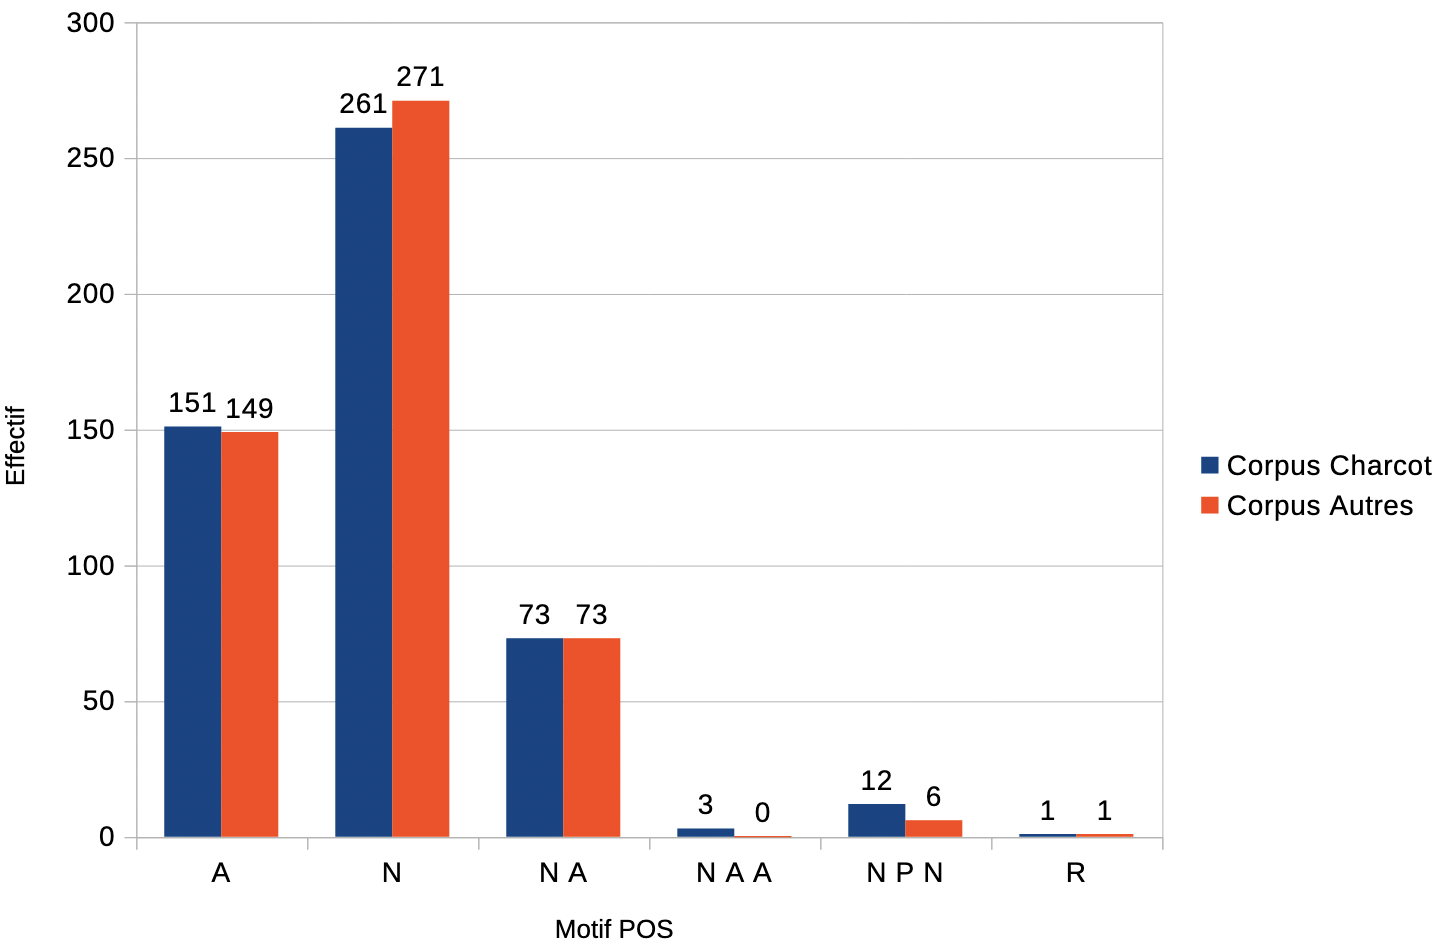
\includegraphics[width=\linewidth]{img/repartition_motifs_POS.png}
	\caption{Analyse comparative des séquences syntaxiques constituant les termes scientifiques dans le corpus \og{}Charcot\fg{} et \og{}Autres\fg{}.}
	\label{fig:repartition_POS}
\end{figure}

Toutefois, \texttt{TermSuite} donne la possibilité d'analyser la pertinence des termes à travers les mesures statistiques. Pour ce qui est de celle de \textsc{TF-IDF},
%une corrélation linéaire positive forte avec le coefficient de détermination \textsc{R}\textsuperscript{2} de $0,93$ (situé dans l'intervalle $[-1, 1]$) a été constatée entre la fréquence brute et la mesure \textsc{TF-IDF} des termes dans le corpus \og{}Charcot\fg{} (indiquée en rouge sur la figure \ref{fig:correlation_Charcot}). 
%Autrement dit, plus un terme est fréquent, plus il est considéré comme pertinent selon la mesure \textsc{TF-IDF}. 
elle mesure la pertinence d'un terme en calculant sa fréquence brute moins l'inverse de sa fréquence documentaire (le nombre de documents contenant ce terme indique sa dispersion). L'intuition derrière cette mesure se résumerait ainsi : si un terme apparaît souvent dans quelques documents, il s'agit d'un terme spécialisé. En revanche, si un terme apparaît souvent dans beaucoup de documents, il sera moins pertinent (un exemple classique de ce phénomène sont les mots vides, p. ex. \textit{par exemple}). 
%La moyenne indiquée par la ligne verte représente la répartition des valeurs \textsc{TF-IDF} normalisées entre $0$ et $1$ autour de leur valeur centrale (\textsc{0,09}), tandis que la médiane (\textsc{0,04}), indiqué en bleu clair, sépare les données en deux groupes égaux. 
%Les valeurs \textsc{TF-IDF} sont inférieures dans le cas des bigrammes et des trigrammes dans le corpus \og{}Charcot\fg{}, contrairement aux unigrammes qui sont classés comme plus pertinents. Par exemple, \textit{pathologie nerveuse} et \textit{cas de paralysie} sont le bigramme et le trigramme les mieux classés avec leurs valeurs de \textsc{TF-IDF} de $0,33$ et de $0,05$, respectivement.
Nous remarquons que les bigrammes comme, p. ex. \textit{paralysie générale} ($0,53$) et \textit{lame médullaire} ($0,51$) n'ont été sous-valorisés dans aucun corpus par rapport aux unigrammes selon cette mesure, puisqu'ils figurent dans les parties supérieures des listes des termes extraites. Cela ne s'applique pas aux trigrammes comme \textit{troubles de sensibilité} ($0,10$) et \textit{pli de passage} ($0,14$). Enfin, nous avons également récupéré les résultats de la spécificité des termes extraits. Cette mesure se réfère au ratio d'étrangeté (angl. \textit{weirdness ratio}) \citep{khurshid2000weirdness}, soit à la \og{}termicité\fg{} des termes dans le corpus par rapport au langage général. Elle exprime le degré de relation d'un terme avec un domaine spécifique. Par exemple, le terme \textit{atrophie} a une termicité plus élevée ($4,44$) que \textit{maladie nerveuses} ($3,15$) dans le corpus \og{}Charcot\fg{} ; le même rapport est observé pour les termes \textit{atrophie} ($4,38$) et \textit{antécédent personnel} ($3,17$) dans le corpus \og{}Autres\fg{}.

%\begin{figure}[h] % Use [H] to force the figure to stay in place
%	\centering
%	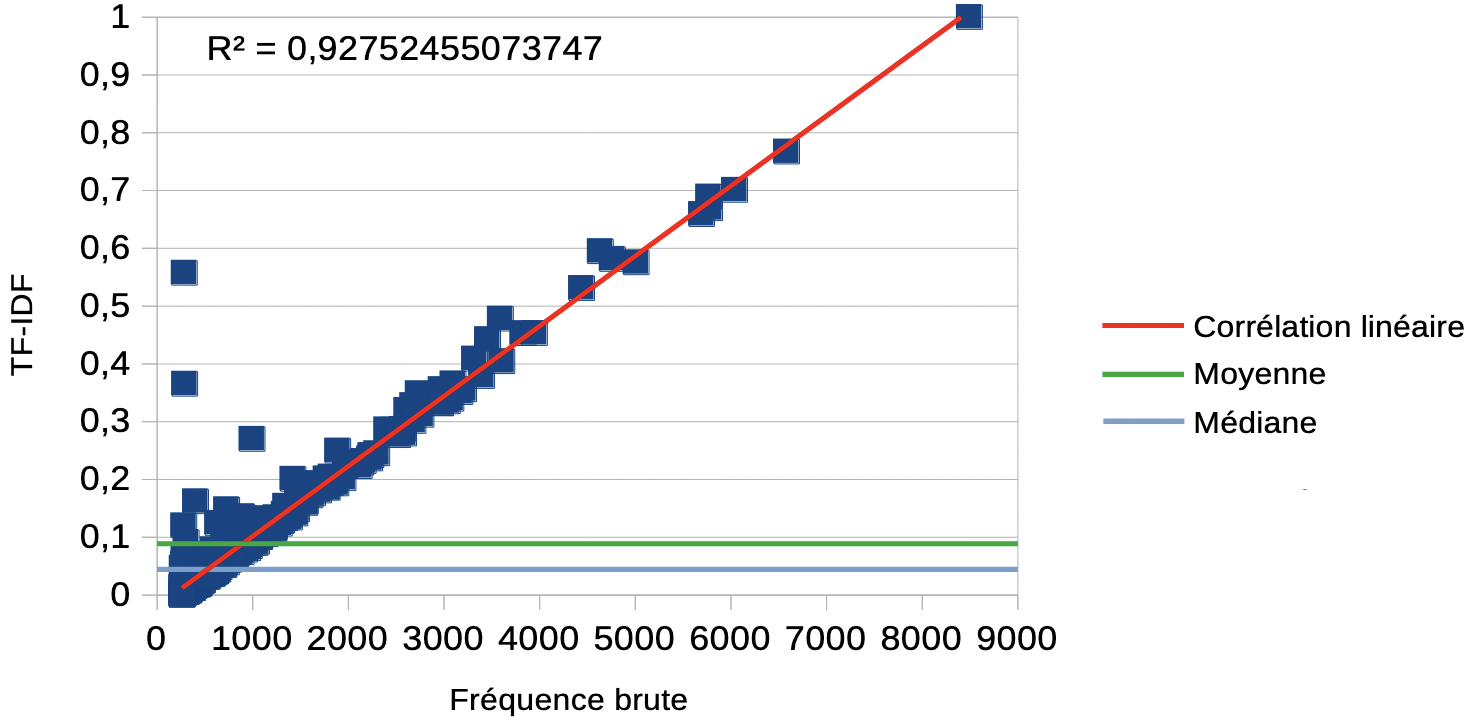
\includegraphics[width=\linewidth]{img/correlation_Charcot.png}
%	\caption{Corrélation linéaire positive entre la fréquence brute et \textsc{TF-IDF} dans le corpus \og{}Charcot\fg{}.}
%	\label{fig:correlation_Charcot}
%\end{figure}

%\begin{figure}[h] % Use [H] to force the figure to stay in place
%	\centering
%	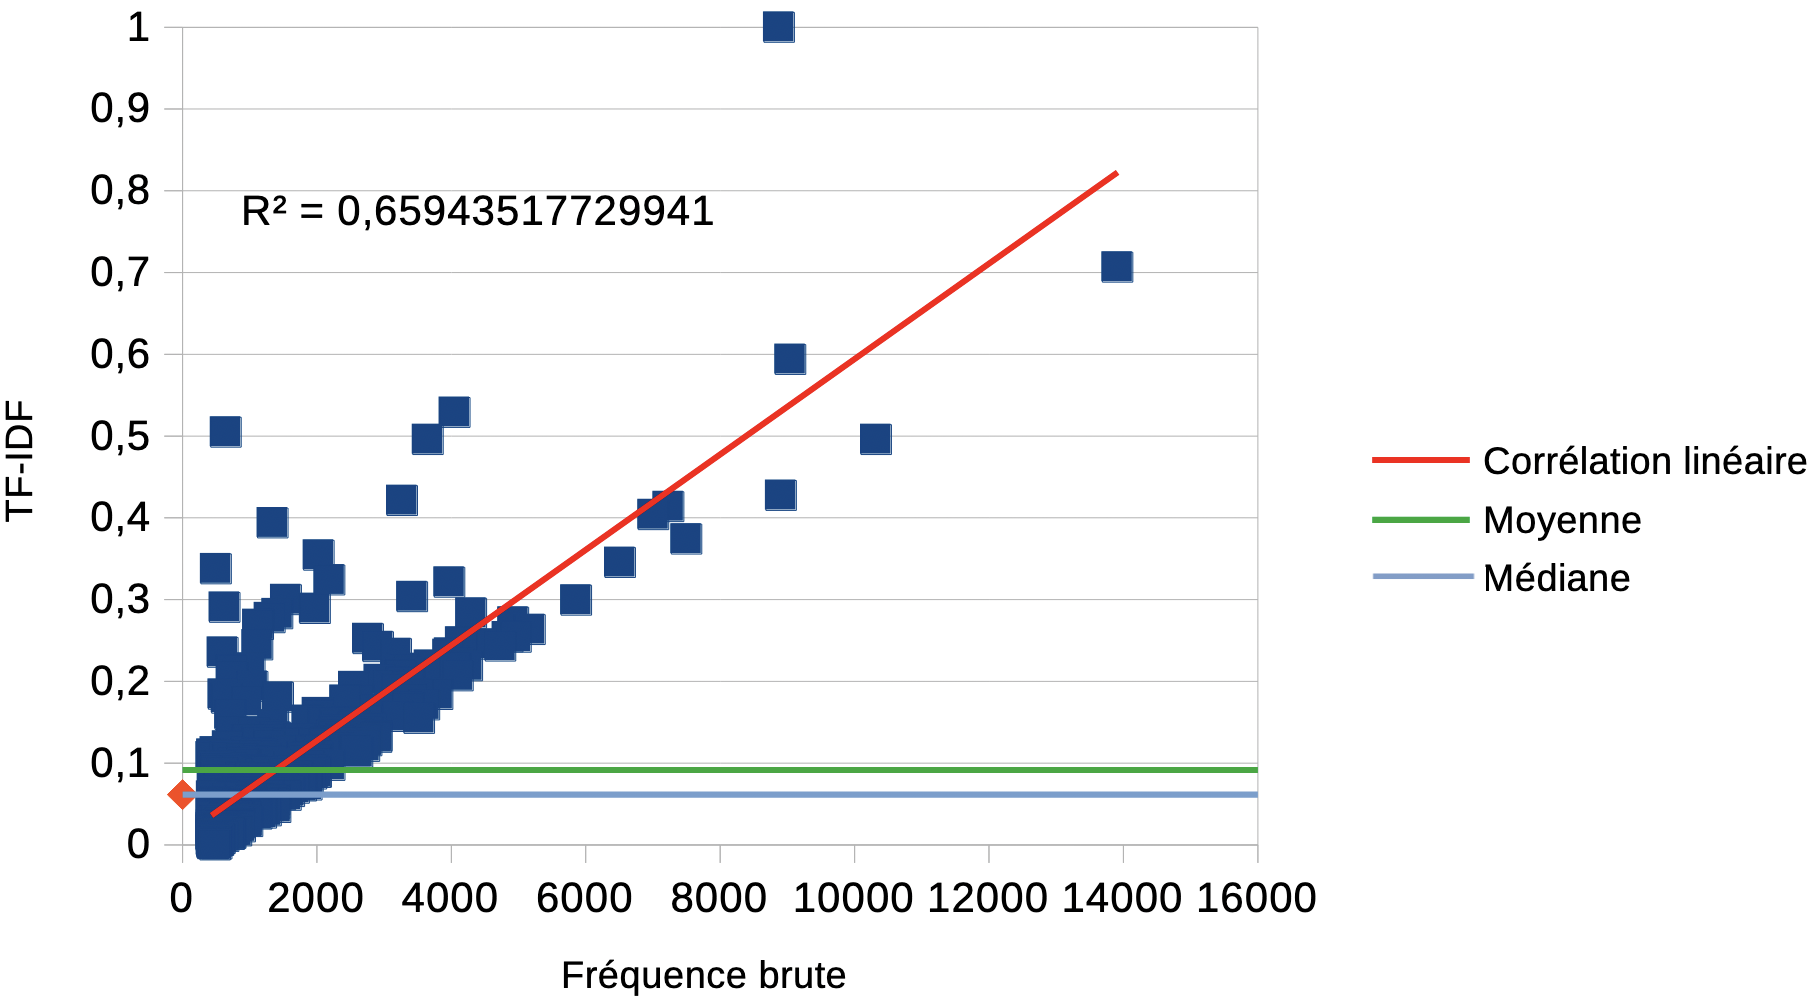
\includegraphics[width=\linewidth]{img/correlation_Autres.png}
%	\caption{Corrélation linéaire positive entre la fréquence brute et \textsc{TF-IDF} dans le corpus \og{}Charcot\fg{}.}
%	\label{fig:correlation_Autres}
%\end{figure}











\section{Extraction des phrases-clés : méthodes statistiques}
\label{sect:methodo_stat}
Afin de surmonter les limites rencontrées avec ces deux outils, nous avons proposé une nouvelle méthode pour identifier des concepts dans les deux corpus en nous basant sur le poids de leur apparition, calculé selon trois différentes mesures de pondération\footnote{Le code est disponible en ligne : \url{https://github.com/ljpetkovic/Charcot\_circulations}.} :
\begin{itemize}
\item \textsc{TF-IDF} est une méthode qui permet d'évaluer l'importance d'un terme contenu dans un document relativement à un corpus plus large en récompensant la fréquence des termes, sans tenir compte des variations de longueur du document ;
\item \textsc{BM25} est une fonction de classement qui classe un ensemble de documents en fonction des termes de requête apparaissant dans chaque document, quelle que soit l'interrelation entre les termes de requête au sein d'un document (par exemple, leur proximité relative). Il s'agit d'une tentative d'amélioration de \textsc{TF-IDF}, notamment pour prendre en compte divers facteurs tels que la longueur du document et les problèmes engendrés par la possible saturation des termes \citep[p.~355]{robertson2009probabilistic} ;
\item \textsc{BERT} \citep{devlin2019} est un modèle pré-entraîné qui utilise l'apprentissage non-supervisé sur de grandes quantités de données textuelles pour apprendre des représentations de mots et de phrases, et comprendre le contexte et la sémantique. Il est basé sur l'architecture des \textit{transformeurs}, qui est un type de grand modèle de langue utilisé pour le \textsc{TAL}.
\end{itemize}

La liste des concepts retenus pour l'étude est composée de termes ou expressions popularisés par Charcot, comme \textit{hystérie}, \textit{sclérose latérale} etc. \citep[p.~1102]{camargo2023} \footnote{\textit{Cf.} la liste exhaustive des termes et des expressions popularisés par Charcot en annexe.}. Pour chaque entrée, nous avons pris en compte les formes du singulier et du pluriel obtenues grâce à des expressions régulières. La liste est  produite de façon supervisée et provient du croisement entre la liste des termes obtenus avec OBVIE et l'index d'une édition des \oe{}uvres complètes de \cite[pp.~493--507]{charcot1892oeuvres}, dont nous avons retiré les termes génériques (\textit{os}, \textit{cerveau}, etc.).

Comme nous pouvons l'observer sur la figure \ref{fig:bm25}, la mesure \textsc{BM25} révèle une intensification du lexique de Charcot dans le corpus \og{}Autres\fg{}. Plus précisément, tous les termes évalués sont identifiés comme plus signifiants dans le discours des \og{}Autres\fg{} que dans celui de Charcot, les scores étant plus élevés pour 14 termes (sur 14 évalués) utilisés par le réseau de Charcot. D'ailleurs, d'après le tableau \ref{tab:calculs_stat} (en annexe), c'est la seule mesure dont les valeurs témoignent clairement d'un lexique partagé entre Charcot et ses successeurs et collaborateurs, \textit{a contrario} des deux autres mesures, où le rapport en question est inversé (la grande majorité des termes étant plus pertinente dans le discours de Charcot, et son impact étant donc moins accentué). Concrètement, les termes les plus pertinents semblent être \textit{sclérose en plaque disséminées} (score 0,83), \textit{paralysie rhumatismale} (0,68), \textit{atrophie progressive} (0,53) et \textit{arthrite déformante} (0,50).
	\begin{table}[h]
	\resizebox{\textwidth}{!}{%
		\centering
		\begin{tabular}{|l|r|r|r|r|}
			\hline
			\rowcolor{gray!10}\multicolumn{1}{|c|}{\textbf{Terme}}
			&	\multicolumn{1}{c|}{\textbf{TF-IDF} (\textit{TermSuite})} & 	\multicolumn{1}{c|}{\textbf{TF-IDF}} & 	\multicolumn{1}{c|}{\textbf{BM25}} & 	\multicolumn{1}{c|}{\textit{\textbf{PatternRank}}} \\
			\hline
			\textit{maladie de Parkinson} & 0,05 & 0,0775 & 0,333 & 0,7936 \\
			\textit{ataxie locomotrice progressive} & 0,32 & 0,0386 & 0,4877 &  0,7431 \\
			\textit{arthropathies tabétiques} & 0,33 & 0,0934 & 0,4928 & 0,7506 \\
			\textit{trépidation épileptoïde du pied} & 0,0198 & 0,1227 & 0,2919 & 0.7597 \\
			\textit{sclérose en plaques disséminées} & NA  & 0,178 & 0,8089 & NA \\
			\textit{tremblement} & NA & 0,1686 & 0,0362 & 0,7683 \\
			\textit{nystagmus} & 0,0243 & 0,1326 & 0,146 & 0,7474 \\
			\textit{embarras parole} & NA & NA & 0,0018 & 0,9347\\
			\textit{sclérose latérale amyotrophique} & NA & 0,044 & 0,6586 & NA \\
			\rowcolor{yellow!30}\textit{tics convulsifs} & NA & 0,1293 & 0,8385 & \textbf{0,8331} \\
			\textit{atrophie musculaire progressive} & 0,40 & 0.1118 & 0.3489 & 0,8053 \\
			%		\textit{abasie} & NA & NA & 0,0445 & 0,3325\\
			\textit{aphasie} & 0,0587 & 0,2245 & 0,1334 & 0,7960 \\
			\textit{astasie-abasie} & NA & 0,0478 & 0,3565 & 0,7375\\
			\textit{athétose} & NA & 0,2029 & 0,274 & 0,8068\\
			\textit{chorées} & NA & 0,1336 & 0,0701 & 0,8047 \\
			\textit{hystérie} & 0,2724 & 0,3711 & 0,0442 & 0,8018 \\
			\textit{épilepsie} & NA & 0,164 & 0,0247 & 0,8199 \\
			\textit{hypnose} & 0,3543 & 1 & 0,2922 & 0,7738 \\
			\hline
		\end{tabular}
	}
	\caption{Les scores de pertinence pour les termes de référence à partir du corpus \og{}Autres\fg{}.}
\end{table}

\begin{figure}[!h]
    \centering
    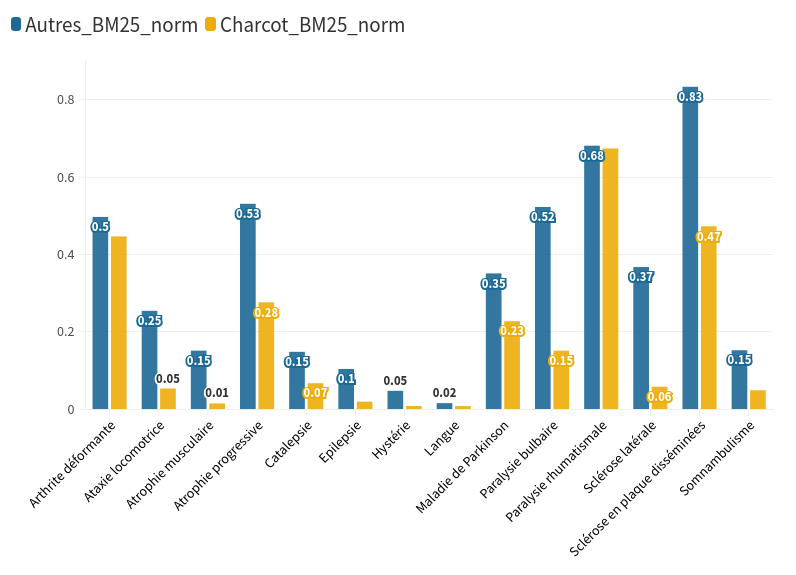
\includegraphics[width=1\textwidth]{img/Charcot_Autres_250523.png}
    \caption{Visualisation de pertinence des concepts dans les deux corpus suivant la métrique \textsc{BM25}. Les valeurs des concepts associées au corpus \og{}Autres\fg{} sont représentées en bleu, alors que celles du corpus \og{}Charcot\fg{} en jaune.}
    \label{fig:bm25}
\end{figure}

D'autre part, nous avons utilisé \textsc{BERT} pour mesurer le poids des termes dans les deux corpus. Bien que ce type de modèle ne fournisse pas directement de poids pour les mots, nous pourrions cependant en extraire des informations utiles pour estimer l'importance ou le poids des mots dans les textes. Différentes approches sont généralement utilisées pour obtenir une représentation de l'importance des mots, en exploitant les informations des plongements lexicaux et des mécanismes d'attention \citep{vaswani2023}. Pour ce travail en cours, nous avons utilisé le modèle \texttt{bert-base-multilingual-cased}. Les premiers résultats obtenus se trouvent dans le tableau \ref{tab:calculs_stat} et restent à améliorer. Cependant, nous avons observé que les termes les plus pertinents pour le discours de Charcot étaient ceux qui désignent les noms des différentes pathologies (\textit{diplopie}, \textit{myélite partielle}, \textit{état de mal épileptique}, \textit{paralysie labio-glosso-laryngée} etc.), contrairement à d'autres notions plus abstraites (\textit{vicieuses}, \textit{délire}, \textit{miracle}) qui sont prédominantes dans le corpus
\og{}Autres\fg{} (termes non renseignés dans le tableau en question). La présence de ce dernier type de notion n'est pas étonnant, étant donné que Charcot aborde la question des guérisons miraculeuses dans ses recherches\footnote{Voir notamment son \oe{}uvre \textit{La foi qui guérit} \citep{charcot1897foi}.}. 


%\chapter{Méthodes de l'état de l'art}
\section{Extraction des phrases-clés : méthode à base d'apprentissage profond}
\label{sect:deep_learning}
En complément de la méthode du calcul de pertinence des termes médicaux fournis de manière supervisée (partie \ref{methodo_stat}), nous exposons ici des résultats de l'approche non-supervisée pour extraire des mots/phrases-clés  pertinents à partir de nos deux corpus\footnote{\textit{Cf.} le dépôt GitHub \url{https://github.com/ljpetkovic/Charcot\_KeyBERT\_Keyphrase-Vectorizers/}.}. L'objectif de cette approche est de détecter les termes communs entre les deux corpus et de montrer la répartition des termes les plus pertinents dans le réseau de Charcot. Deux algorithmes librement disponibles sont présentés ici pour illustrer cette dernière approche : \texttt{keybert} et \texttt{keyphrase-vectorizers}. Lors du passage à l'échelle avec la quantité de données considérable (voir le tableau \ref{tab:corpus}), nous avons fait face un manque de puissance de calcul des ordinateurs locaux. Pour faciliter l'extraction des phrases-clés, nous avons obtenu l'accès à la plateforme technologique \textsc{MeSU} et un accompagnement technique grâce à l'unité de service \textsc{SACADO} (Service d'Aide au Calcul et à l'Analyse de Données)\footnote{\url{https://sacado.sorbonne-universite.fr/fr/}.} de Sorbonne Université.

\subsection{Librairie \texttt{keybert}}

Cette librairie Python permet d'exploiter les plongements de mots (angl. \textit{word embeddings}) du type \textsc{BERT} pour générer des mots/phrases-clés les plus similaires à un document.
La figure \ref{fig:keybert} illustre la chaîne de traitement appliquée à nos deux corpus : 
\begin{enumerate}
\item les corpus \og Charcot \fg{} et \og Autres \fg{} sont utilisés comme les données d'entrée au format \texttt{.txt} ;
\item les documents d'entrée ont été tokenisés en phrases-clés candidates avec la fonction \texttt{CountVectorizer} ; 
\item les plongements des documents et de leurs phrases-clés candidates ont été générés par le modèle de langue \texttt{sentence-transformers} ;
\item la similarité cosinus a été calculée entre les documents d'entrée et les phrases-clés candidates, où celles avec les scores les plus élevés sont extraites.
\end{enumerate}

\begin{figure}[!h]
    \centering
    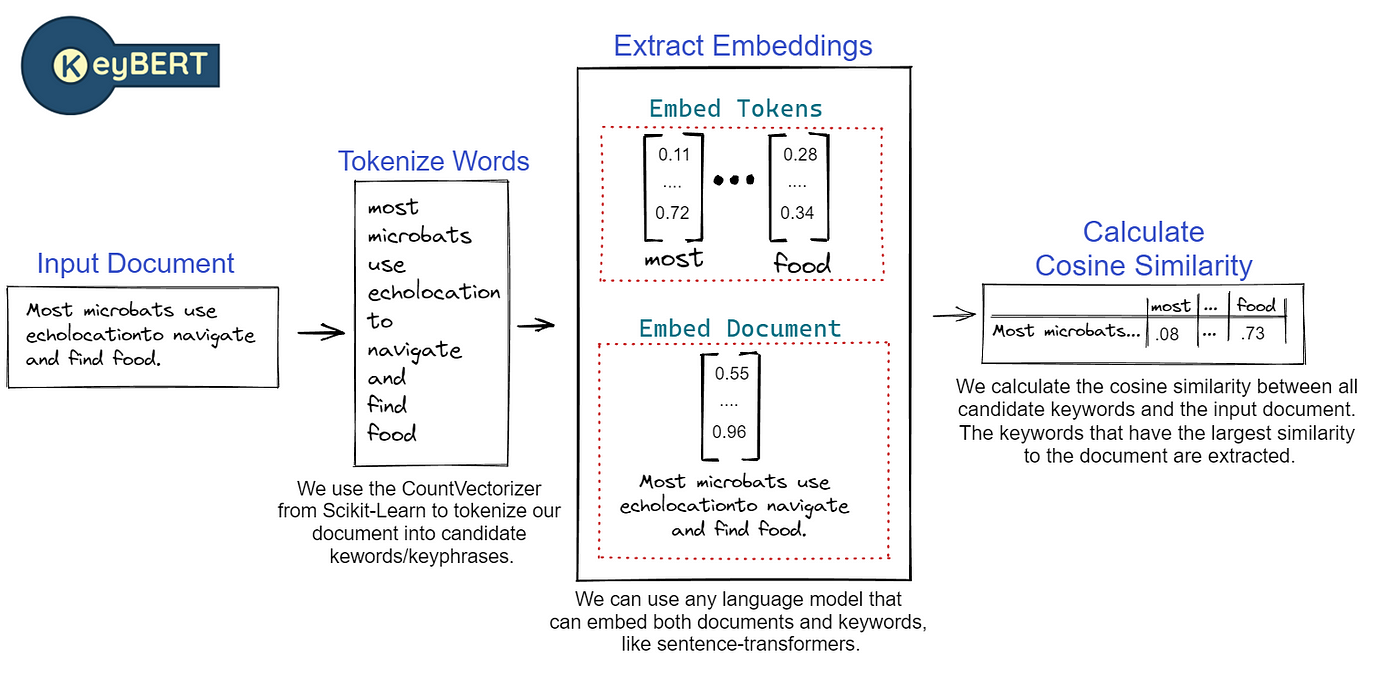
\includegraphics[width=1\textwidth]{img/keybert.png}
    \caption[\textit{Pipeline} de la librairie \texttt{keybert}.]{\textit{Pipeline} de la librairie \texttt{keybert}\protect\footnotemark{.}}
    \label{fig:keybert}
\end{figure}

\footnotetext{Illustration reprise de \url{https://maartengr.github.io/KeyBERT/guides/quickstart.html\#installation}.}

Une première tentative de génération des phrases-clés les plus pertinentes dans les deux corpus n'a produit que deux termes : \textsc{articulation de} [\textit{sic}] \textsc{épaule} et \textsc{paralysie faciale périphérique}. Par ailleurs, en observant les 15 phrases-clés les plus pertinentes dans le corpus \og Autres \fg{} (figure \ref{fig:keybert_autres}), nous constatons un manque de diversification des résultats et des phrases-clés qui se ressemblent (\textit{la sensibilité tactile}, \textit{sensibilité tactile au}, \textit{la sensibilité tend} etc.)\footnote{Pour assurer que les phrases-clés ne se ressemblent pas, il faut utiliser le paramètre \texttt{use\_mmr} et spécifier sa valeur entre 0 et 1.}. Un autre problème observé était la non-grammaticalité des phrases-clés extraites (\textit{sémi lunaire segment}, \textit{prière le malade} etc.), ce qui nous a incités à tester une approche plus fine, décrite dans la partie \ref{patternrank}.

\begin{figure}[!h]
    \centering
    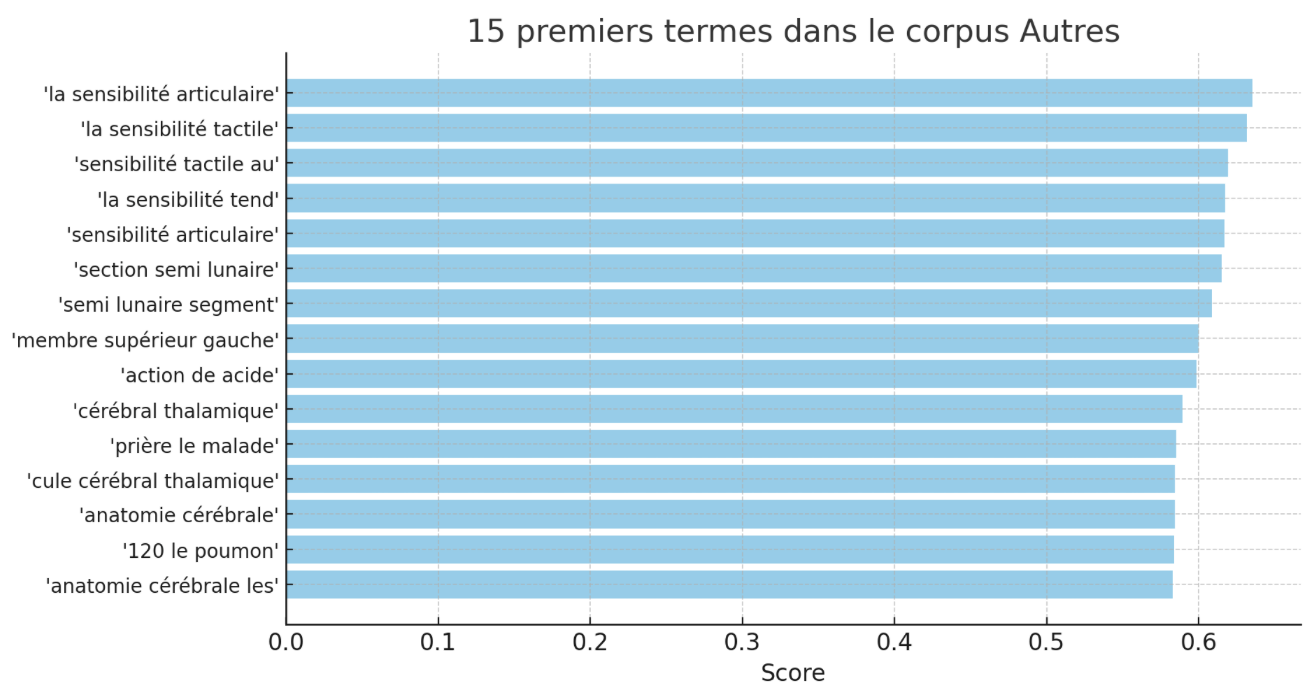
\includegraphics[width=1\textwidth]{img/keybert_autres.png}
    \caption{Répartition des 15 termes les plus pertinents dans le corpus \og{}Autres\fg{} selon \texttt{keybert}.}
    \label{fig:keybert_autres}
\end{figure}


\subsection{Approche \textit{PatternRank}}
\label{patternrank}
Cette approche exploite la librairie \texttt{keyphrase-vectorizers} qui offre la possibilité d'extraire les phrases-clés pertinentes et spécifiques à l'aide des balises de parties de discours. Cela nous a paru comme une piste intéressante, étant donné que les termes médicaux (surtout ceux plus pointus) que l'on souhaitait extraire étaient généralement des n-grammes constitués des substantifs, suivis d'un ou plusieurs adjectifs (p. ex. \textit{sclérose latérale amyotrophique}). Voici les étapes de la chaîne de traitement de l'approche \textit{PatternRank} (figure \ref{fig:patternrank}) :
\begin{enumerate}
\item les corpus \og Charcot \fg{} et \og Autres \fg{} sont utilisés comme les données d'entrée au format \texttt{.txt} ;
\item les tokens ont été extraits et étiquetés avec les balises de partie du discours et les expressions régulières \texttt{<N.*>+<ADJ.*>*} (sans utiliser le paramètre \texttt{use\_mmr}) ;
\item les tokens ont été sélectionnés selon les balises de partie de discours souhaitées et gardés comme les phrases-clés candidates ;
\item les plongements des documents et de leurs phrases-clés candidates ont été générés par le modèle de langue (en l'occurrence \texttt{flair}\footnote{\url{https://github.com/flairNLP/flair}}) ;
\item les similarités cosinus ont été calculées entre ces deux types de plongements, et les phrases-clés candidates ont été triées par ordre décroissant ;
\item les phrases-clés les plus représentatives ont été extraites.
\end{enumerate}

\begin{figure}[!h]
    \centering
    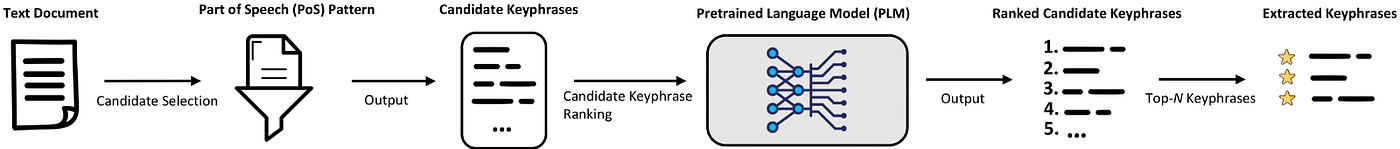
\includegraphics[width=1\textwidth]{img/patternrank_workflow.png}
    \caption{\textit{Workflow} de la méthode \textit{PatternRank} \citep[p.~2]{schopf2022}.}
    \label{fig:patternrank}
\end{figure}

La figure \ref{fig:patternrank_partage} nous informe sur les 15 termes les plus pertinents et fréquents, extraits avec la librairie \texttt{keyphrase-vectorizers}, que l'on retrouve dans les deux corpus. Malgré certains tokens tronqués, très probablement en raison d'un \textsc{OCR} imparfait (\textit{ments} $\rightarrow$ \textit{mouvements}, \textit{decins} $\rightarrow$ \textit{médecins} etc.), nous observons une diversification des résultats. Après cela, il reste la question de mieux comprendre le rôle des phrases-clés extraites dans les écrits de l'entourage de Charcot et/ou si elles sont vraiment significatives ou pas. 

\begin{figure}[!h]
    \centering
    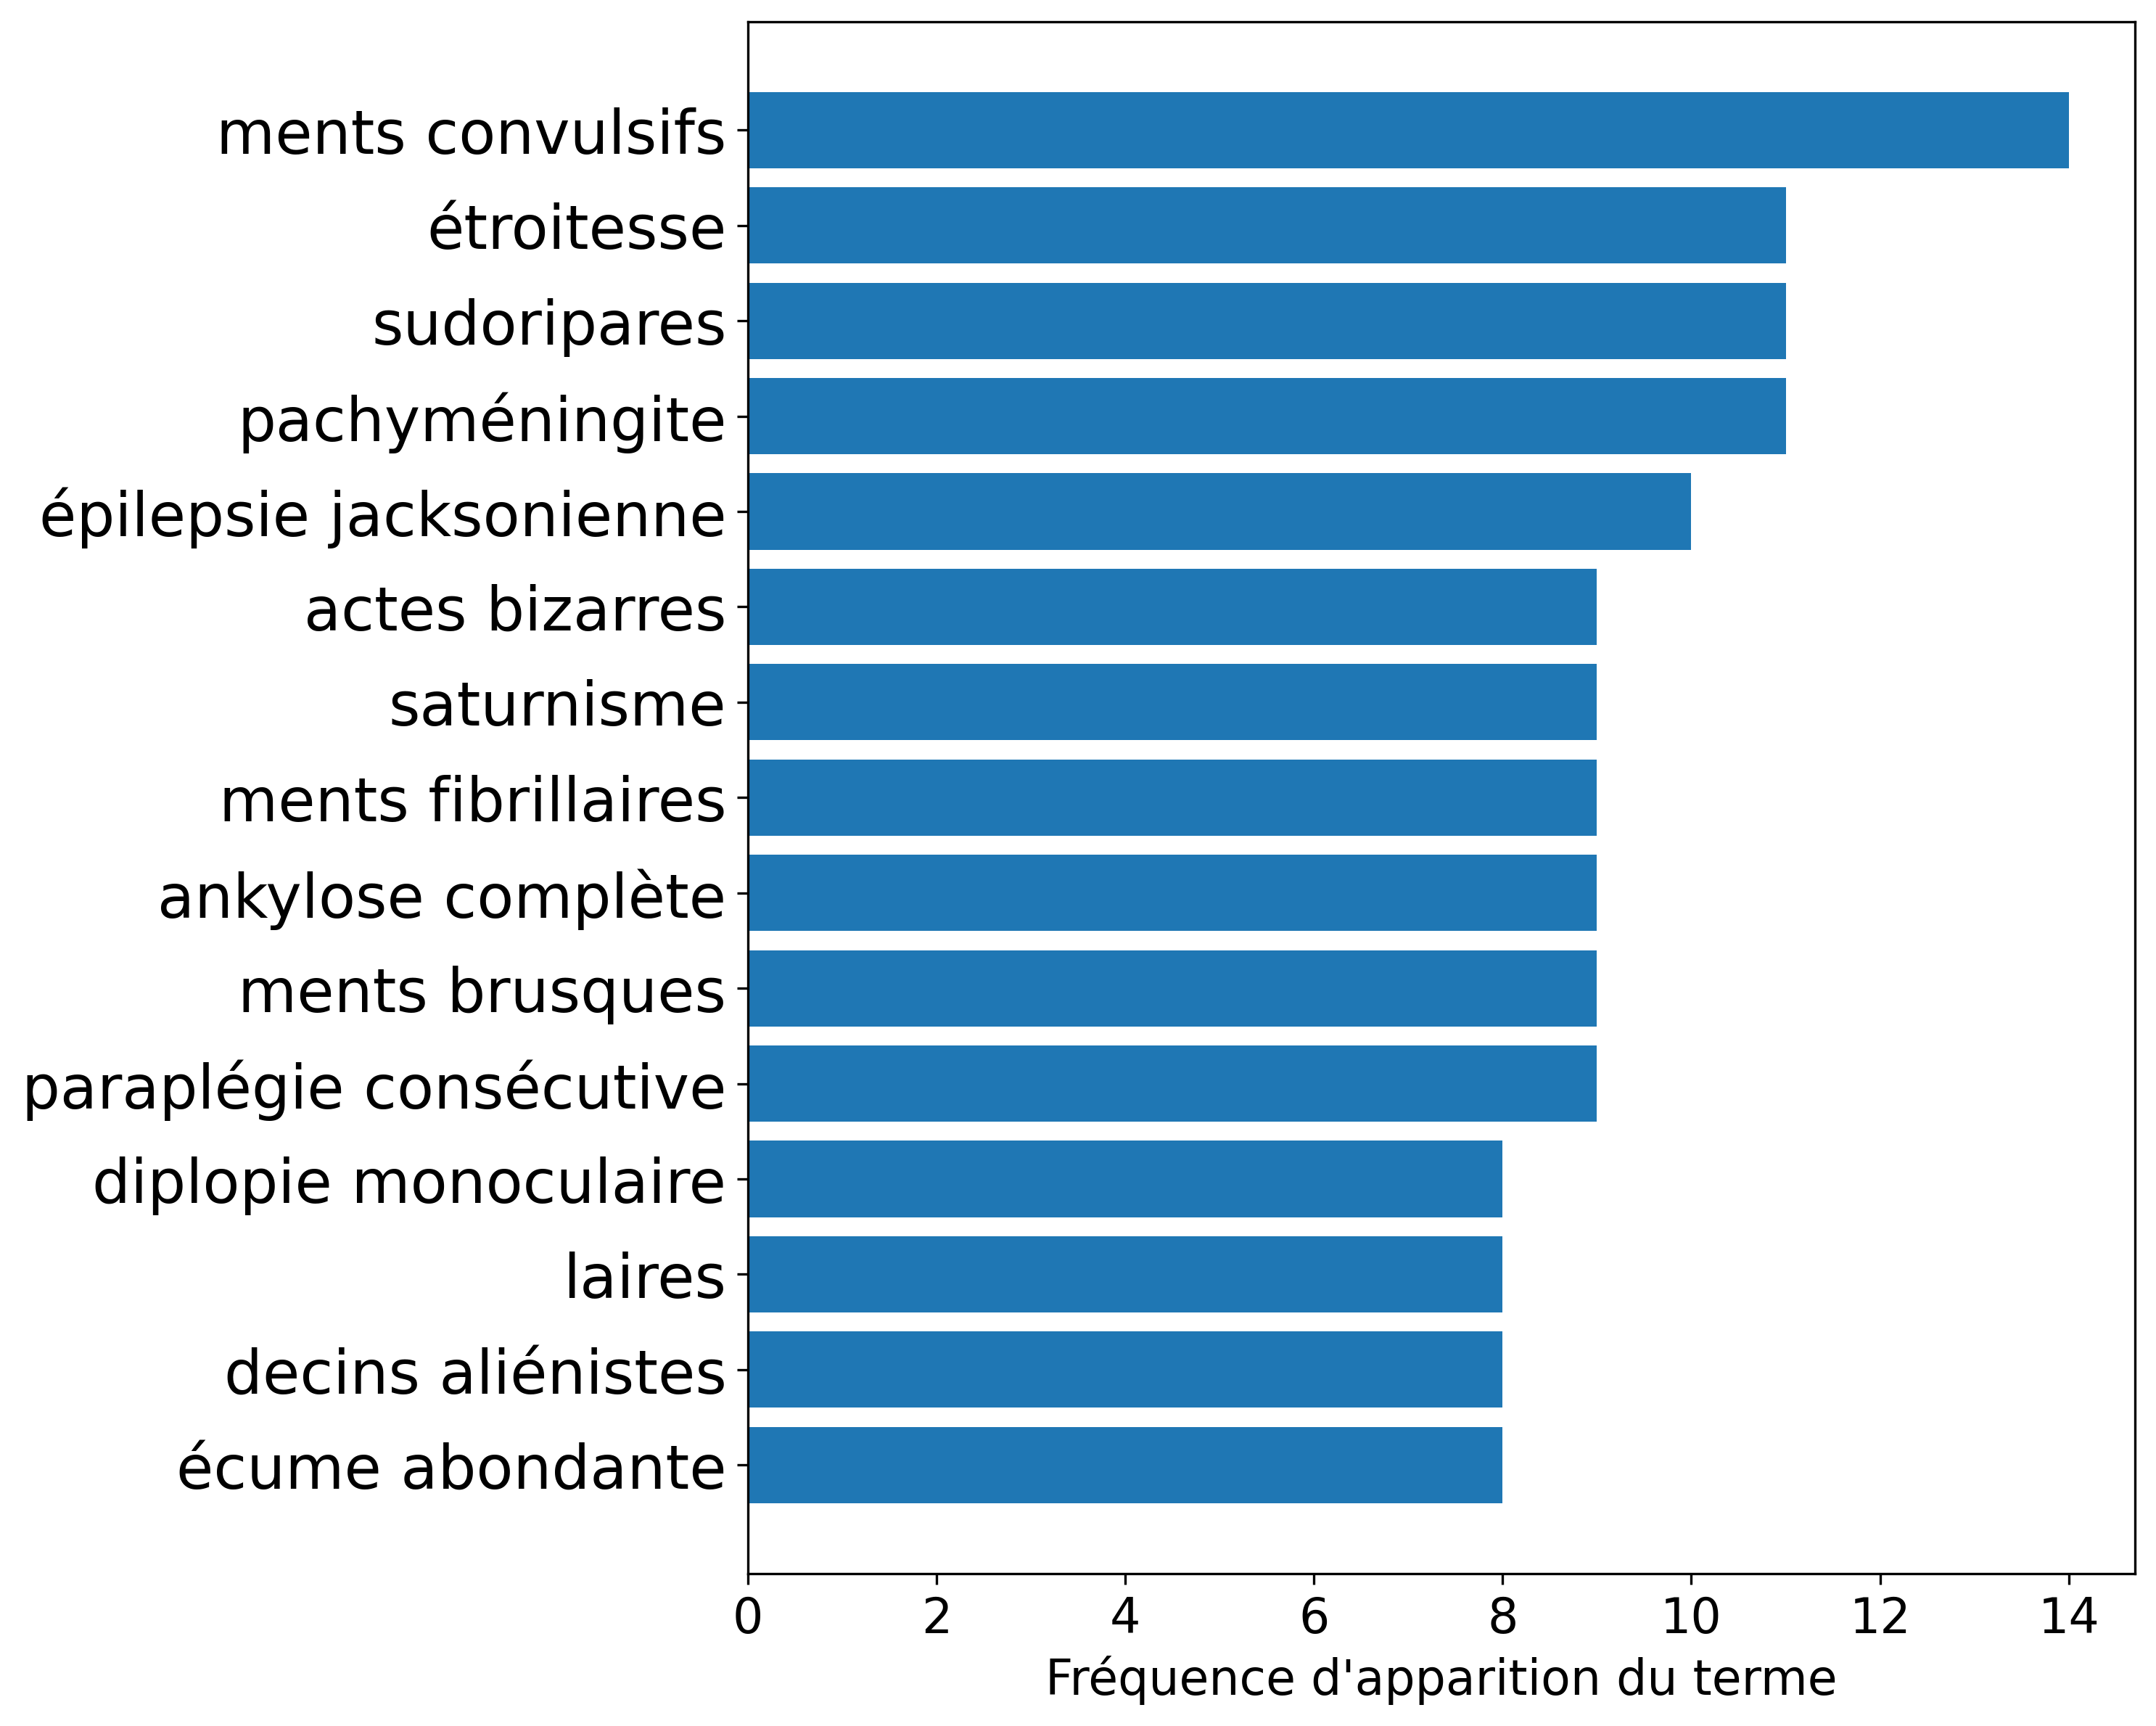
\includegraphics[width=1\textwidth]{img/termes_partages.png}
    \caption{Les 15 termes les plus fréquents partagés par les deux corpus selon \texttt{keyphrase-vectorizers}.}
    \label{fig:patternrank_partage}
\end{figure}

\section{L'estimation de l'impact de l'entité \texttt{Jean-Martin Charcot} à l'aide de l'outil Rankingdom}
\label{sect:rankingdom}
\hl{à intégrer dans la rédaction}

\hl{À retravailler}

comme présenté dans le tableau \ref{tab:rankingdom} : ces métriques sont calculées pour l'entité \texttt{Jean-Martin Charcot}.

\begin{table}[htbp]
	\centering
	\footnotesize
	\resizebox{\textwidth}{!}{ % Resize the table to fit within text width
		\begin{tabular}{|c|c|c|}
			\hline
			\rowcolor{maroon!10}
			\begin{tabular}[c]{@{}c@{}}\textit{Métrique}\end{tabular} & \begin{tabular}[c]{@{}c@{}}\textit{Définition}\end{tabular}                                                                                         & \begin{tabular}[c]{@{}c@{}}\textit{Exemple}\end{tabular}                                                                                                                                             \\
			\hline
			\begin{tabular}[c]{@{}c@{}}\textsc{Portée}\\ (\textsc{Popularité})\end{tabular} & \begin{tabular}[c]{@{}l@{}}nombre d'assertions décrivant une entité\end{tabular}                                                                                         & Charcot est décrit par 546 assertions.                                                                                                                                                \\
			\hline
			\textsc{Influence}                                                     & \begin{tabular}[c]{@{}l@{}}nombre d'entités liées à une entité\end{tabular}                                                                                        & 191 entités liées à Charcot.                                                                                                                                                     \\
			\hline
			\textsc{À propos}                                                      & \begin{tabular}[c]{@{}l@{}}nombre d'entités impactées \\ (\oe{}uvres originales, évènements$\dots$)\end{tabular}                                                                    & 56 entités à propos de Charcot.                                                                                                                                                  \\
			\hline
			\textsc{Indice \textit{a}}                                                       & \begin{tabular}[c]{@{}c@{}}nombre maximum d'entités impactées \textit{a} \\
				ayant le comptage \og{} à propos \fg{}\end{tabular} & \begin{tabular}[c]{@{}c@{}}13 entités impactées par Charcot ont \\ le comptage \og{} à propos \fg{} supérieur à 13.\end{tabular} \\
			\hline
			\textsc{Impact}                                                        & \begin{tabular}[c]{@{}c@{}}somme de tous les comptages \og{} à propos \fg{}\\
				de toutes les entités impactées\end{tabular}               & L'impact de Charcot est 826.                                                                                                                                                         \\
			\hline
		\end{tabular}
	}
	\caption{Aperçu des métriques Rankingdom pour quantifier l'importance de l'entité \texttt{Jean-Martin Charcot}.}
	\label{tab:rankingdom}
\end{table}

De plus, des calculs effectués à partir de la portée et de l'influence de Charcot permettent de générer un graphique de \og{}quadrant magique de Gartner\fg{} (angl. \textit{Gartner Magic Quadrant})\footnote{Le nom provient de la société américaine de conseil Gartner qui \og{}publie chaque année les résultats de ses analyses dans plus de 100 secteurs technologiques\fg{} \citep{gartner}.}. Cette représentation sur la figure \ref{fig:analyse_quadrant} met en valeur quatre types d'entités : 
\begin{itemize}
	\item \textbf{acteurs de niche} : entités avec une portée et une influence modestes (p. ex. Pierre Marie) ;
	\item \textit{\textbf{challengers}} : entités ayant une certaine reconnaissance et une influence considérable, mais qui sont de taille mineure, more concentrées, avec une portée plus petite (Charles-Joseph Bouchard) ;
	\item \textbf{visionnaires} : entités avec une grande portée, dont l'influence reste néanmoins limitée et qui recevront plus de reconnaissance ultérieurement (Paul Richer) ;
	\item \textit{\textbf{leaders}} : entités les plus importantes, avec une grande portée, connues à grande échelle et dans plusieurs domaines, tout en étant reconnues comme ayant une grande influence (Charcot).
\end{itemize}

\begin{figure}[htpb]
	\centering
	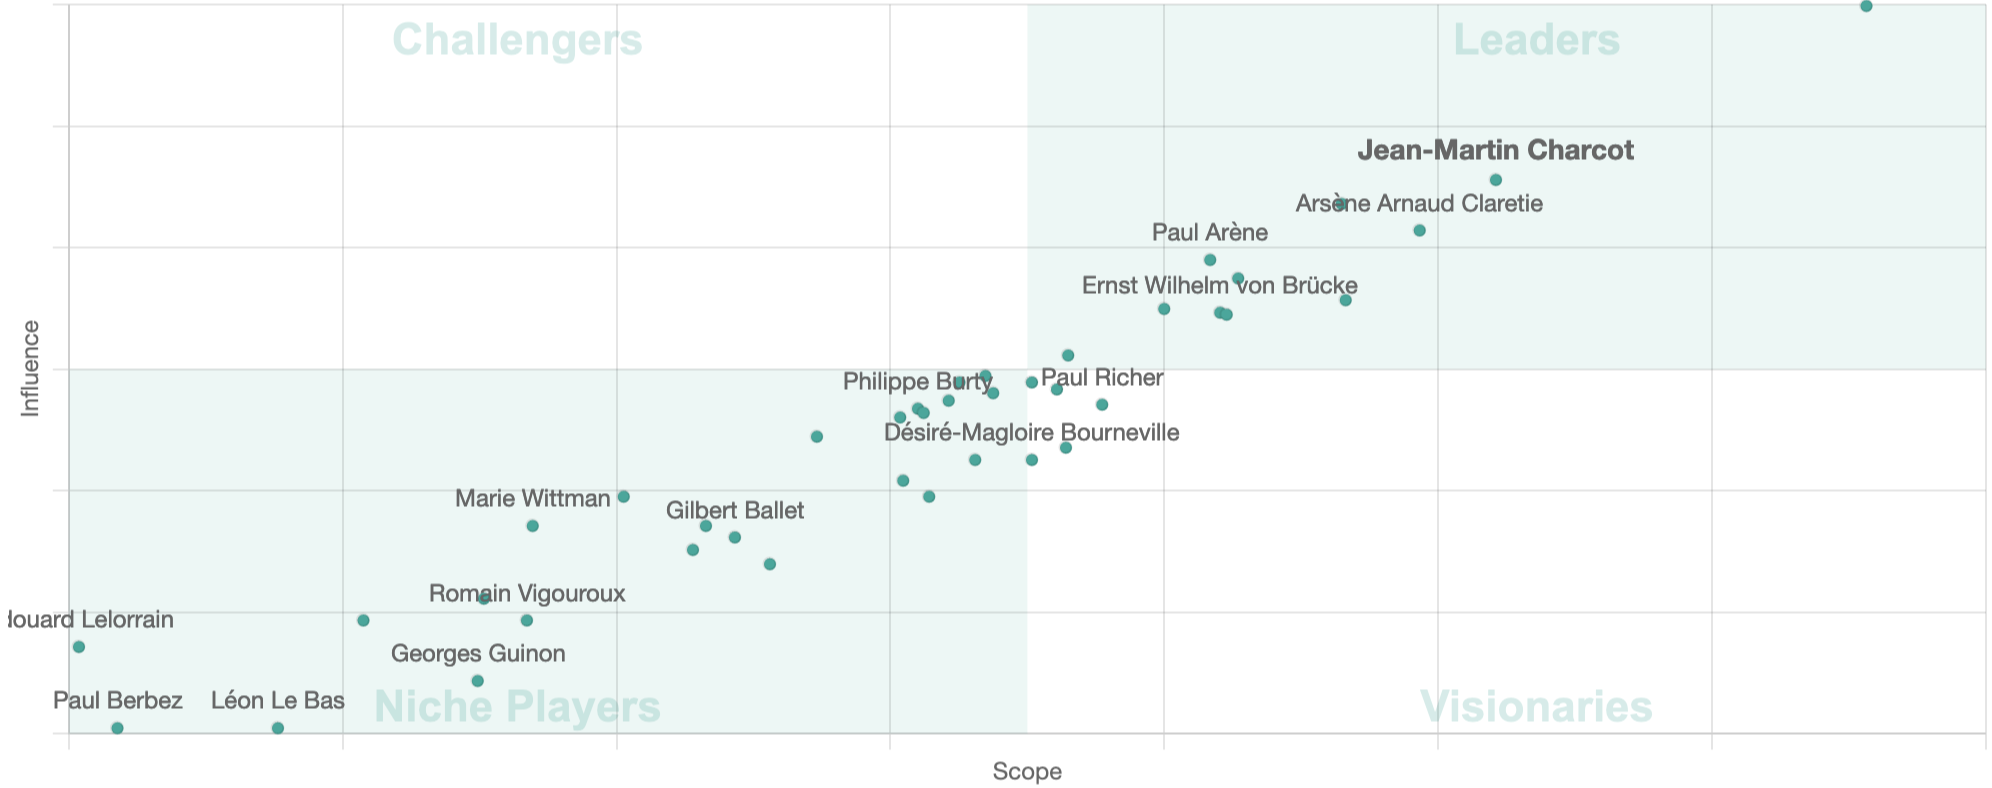
\includegraphics[width=1\textwidth]{img/analyse_quadrant.png}
	\caption[Positionnement de l'entité \texttt{Jean-Martin Charcot} au sein de son domaine et comparaison avec les entités les plus similaires à lui \textit{via} une analyse de quadrant de l'outil Rankingdom.]{Positionnement de l'entité \texttt{Jean-Martin Charcot} au sein de son domaine et comparaison avec les entités les plus similaires à lui \textit{via} une analyse de quadrant de l'outil Rankingdom\protect\footnotemark{.}}
	% Pour raison de visibilité, l'image originale a été agrandie, ce qui a entraîné le rapprochement des années sur l'axe de l'abscisse.
	\label{fig:analyse_quadrant}
\end{figure}

\footnotetext{\url{https://www.rankingdom.org/entity/Q20710?search=jean-martin+charcot}. Le domaine dans lequel Charcot figure est relativement large, y compris les figures du domaine médical (p. ex. Bourneville), mais aussi littéraire (Arsène Arnaud Claretie).}

\bigskip
L'impact de Charcot peut également être visualisé à l'aide de Rankingdom à travers le graphique qui apporte une dimension temporelle (figure \ref{fig:impact_temporel}). Il s'agit notamment de la cumulation temporelle de son impact, où l'on peut observer qu'il s'étend sur la période 1856--1994. 

\begin{figure}[h]
	\centering
	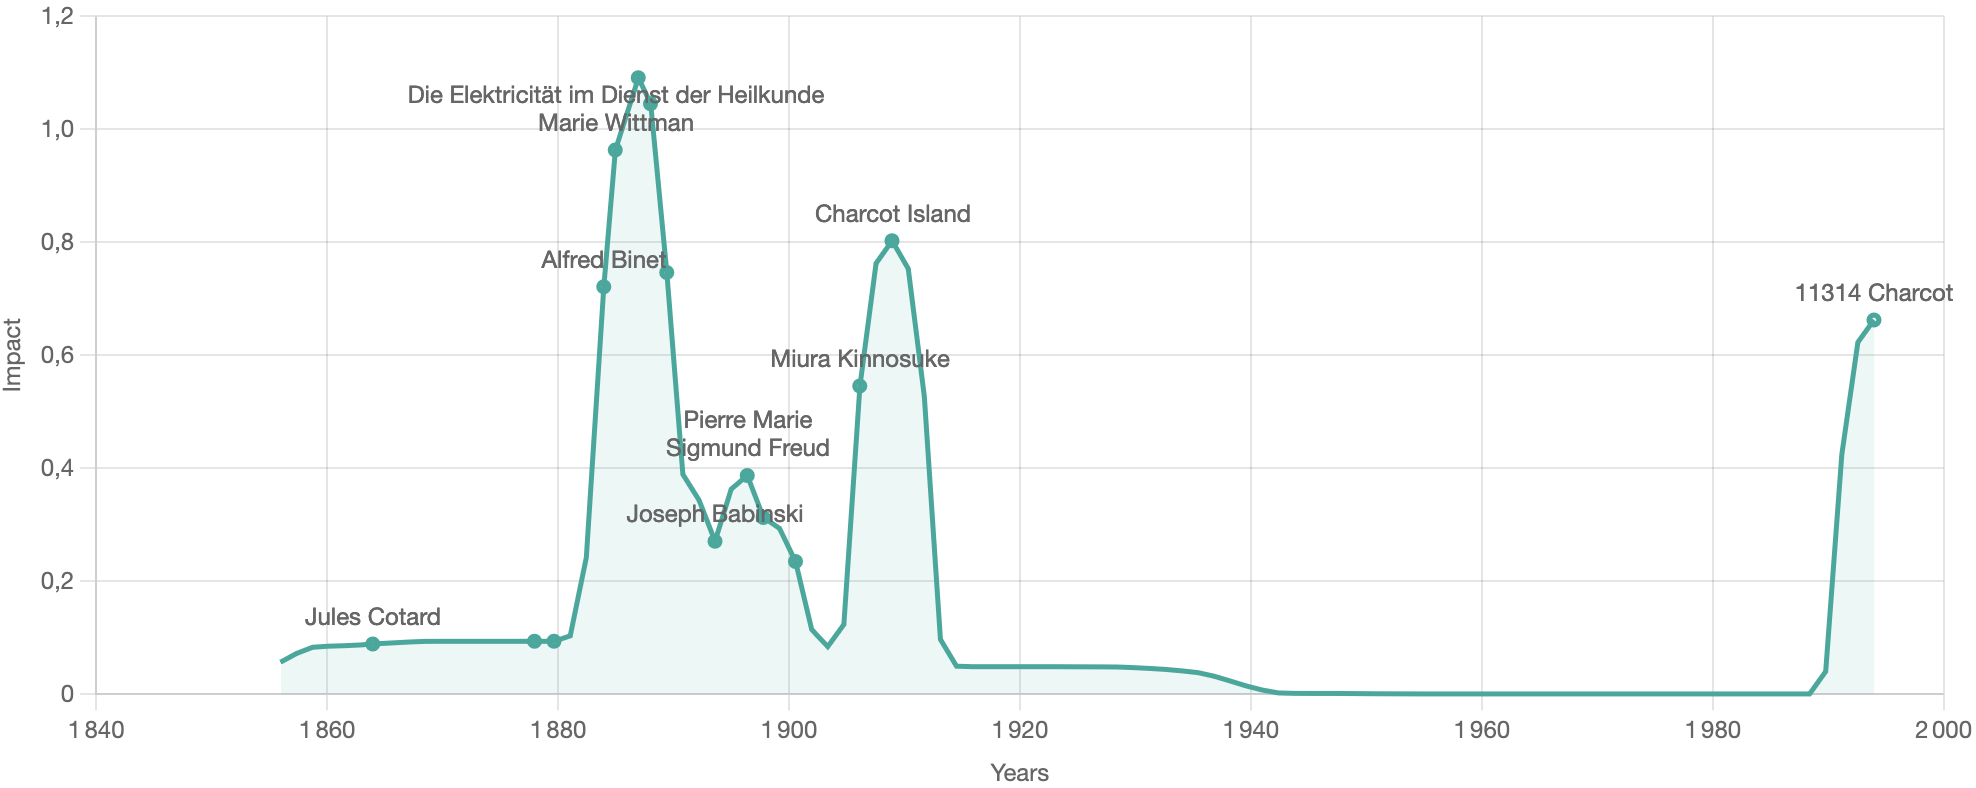
\includegraphics[width=1\textwidth]{img/impact_temporel.png}
	\caption[Analyse temporelle de l'impact de l'entité \texttt{Jean-Martin Charcot} à l'aide de l'outil Rankingdom.]{Analyse temporelle de l'impact de l'entité \texttt{Jean-Martin Charcot} à l'aide de l'outil Rankingdom\protect\footnotemark{.}}
	% Pour raison de visibilité, l'image originale a été agrandie, ce qui a entraîné le rapprochement des années sur l'axe de l'abscisse.
	\label{fig:impact_temporel}
\end{figure}

\footnotetext{\url{https://www.rankingdom.org/entity/Q20710?search=jean-martin+charcot}.}

Enfin, il est également possible de lister les entités impactées, comprenant les personnes (p. ex. Sigmund Freud), les notions médicales (SEP) ou bien les entités géographiques afférentes (Île Charcot).

\section{Évaluation qualitative}
\label{sect:eval_quali}
